%\VignetteEngine{knitr::knitr}
%% LyX 2.1.4 created this file.  For more info, see http://www.lyx.org/.
%% Do not edit unless you really know what you are doing.
\documentclass{article}
\usepackage[sc]{mathpazo}
\usepackage[T1]{fontenc}
\usepackage{geometry}
\geometry{verbose,tmargin=2.5cm,bmargin=2.5cm,lmargin=2.5cm,rmargin=2.5cm}
\setcounter{secnumdepth}{2}
\setcounter{tocdepth}{2}
\usepackage{url}
\usepackage[utf8]{inputenc}
\usepackage[unicode=true,pdfusetitle,
 bookmarks=true,bookmarksnumbered=true,bookmarksopen=true,bookmarksopenlevel=2,
 breaklinks=false,pdfborder={0 0 1},backref=false,colorlinks=false]
 {hyperref}
\hypersetup{
 pdfstartview={XYZ null null 1}}
\begin{document}



\title{Epistatic Nested Effects Models\\
	Inferring mixed epistatis from indirect measurements of knockout screens.}


\author{Madeline, Diekmann \& Martin Pirkl}

\maketitle
This package is an extension of the classic Nested Effects Models provided in package \emph{nem}. Nested Effects Models is a pathway reconstruction method, which takes into account effects of downstream genes. Those effects are observed for every knockout of a pathway gene, and the nested structure of observed effects can then be used to reconstruct the pathway structure.
However, classic Nested Effects Models do not account for double knockouts. In this package \emph{epiNEM}, one additional layer of complexity is added. For every two genes, acting on one gene together, the relationship is evaluated and added to the model as a logic gate. Genetic relationships are represented by the logics OR (no relationship), AND (functional overlap), NOT (masking or inhibiting) and XOR (mutual prevention from acting on gene C).

\section*{Loading epiNEM}

\begin{knitrout}
\definecolor{shadecolor}{rgb}{0.969, 0.969, 0.969}\color{fgcolor}\begin{kframe}
\begin{alltt}
\hlcom{## install.packages("devtools", verbose = F, quiet = T)}

\hlkwd{library}\hlstd{(devtools)}

\hlcom{## install_github("cbg-ethz/epiNEM", quiet = T)}

\hlkwd{library}\hlstd{(epiNEM)}
\end{alltt}
\end{kframe}
\end{knitrout}

\section*{Simulations}
We compare epiNEM to several network inference methods.

\begin{knitrout}
\definecolor{shadecolor}{rgb}{0.969, 0.969, 0.969}\color{fgcolor}\begin{kframe}
\begin{alltt}
\hlkwd{library}\hlstd{(bnem)} \hlcom{# MartinFXP/B-NEM/package}
\end{alltt}


{\ttfamily\noindent\itshape\color{messagecolor}{\#\# Loading required package: CellNOptR}}

{\ttfamily\noindent\itshape\color{messagecolor}{\#\# Loading required package: RBGL}}

{\ttfamily\noindent\itshape\color{messagecolor}{\#\# Loading required package: graph}}

{\ttfamily\noindent\itshape\color{messagecolor}{\#\# Loading required package: BiocGenerics}}

{\ttfamily\noindent\itshape\color{messagecolor}{\#\# Loading required package: parallel}}

{\ttfamily\noindent\itshape\color{messagecolor}{\#\# \\\#\# Attaching package: 'BiocGenerics'}}

{\ttfamily\noindent\itshape\color{messagecolor}{\#\# The following objects are masked from 'package:parallel':\\\#\# \\\#\#\ \ \ \  clusterApply, clusterApplyLB, clusterCall, clusterEvalQ, clusterExport,\\\#\#\ \ \ \  clusterMap, parApply, parCapply, parLapply, parLapplyLB, parRapply,\\\#\#\ \ \ \  parSapply, parSapplyLB}}

{\ttfamily\noindent\itshape\color{messagecolor}{\#\# The following objects are masked from 'package:igraph':\\\#\# \\\#\#\ \ \ \  normalize, union}}

{\ttfamily\noindent\itshape\color{messagecolor}{\#\# The following objects are masked from 'package:stats':\\\#\# \\\#\#\ \ \ \  IQR, mad, xtabs}}

{\ttfamily\noindent\itshape\color{messagecolor}{\#\# The following objects are masked from 'package:base':\\\#\# \\\#\#\ \ \ \  anyDuplicated, append, as.data.frame, cbind, colnames, do.call, duplicated,\\\#\#\ \ \ \  eval, evalq, Filter, Find, get, grep, grepl, intersect, is.unsorted, lapply,\\\#\#\ \ \ \  lengths, Map, mapply, match, mget, order, paste, pmax, pmax.int, pmin,\\\#\#\ \ \ \  pmin.int, Position, rank, rbind, Reduce, rownames, sapply, setdiff, sort,\\\#\#\ \ \ \  table, tapply, union, unique, unsplit}}

{\ttfamily\noindent\itshape\color{messagecolor}{\#\# \\\#\# Attaching package: 'graph'}}

{\ttfamily\noindent\itshape\color{messagecolor}{\#\# The following objects are masked from 'package:igraph':\\\#\# \\\#\#\ \ \ \  degree, edges, intersection}}

{\ttfamily\noindent\itshape\color{messagecolor}{\#\# \\\#\# Attaching package: 'RBGL'}}

{\ttfamily\noindent\itshape\color{messagecolor}{\#\# The following objects are masked from 'package:igraph':\\\#\# \\\#\#\ \ \ \  bfs, dfs, transitivity}}

{\ttfamily\noindent\itshape\color{messagecolor}{\#\# The following object is masked from 'package:e1071':\\\#\# \\\#\#\ \ \ \  extractPath}}

{\ttfamily\noindent\itshape\color{messagecolor}{\#\# Loading required package: hash}}

{\ttfamily\noindent\itshape\color{messagecolor}{\#\# hash-2.2.6 provided by Decision Patterns}}

{\ttfamily\noindent\itshape\color{messagecolor}{\#\# Loading required package: ggplot2}}

{\ttfamily\noindent\itshape\color{messagecolor}{\#\# Loading required package: RCurl}}

{\ttfamily\noindent\itshape\color{messagecolor}{\#\# Loading required package: bitops}}

{\ttfamily\noindent\itshape\color{messagecolor}{\#\# Loading required package: Rgraphviz}}

{\ttfamily\noindent\itshape\color{messagecolor}{\#\# Loading required package: grid}}

{\ttfamily\noindent\itshape\color{messagecolor}{\#\# Loading required package: XML}}

{\ttfamily\noindent\itshape\color{messagecolor}{\#\# \\\#\# Attaching package: 'XML'}}

{\ttfamily\noindent\itshape\color{messagecolor}{\#\# The following object is masked from 'package:graph':\\\#\# \\\#\#\ \ \ \  addNode}}

{\ttfamily\noindent\itshape\color{messagecolor}{\#\# Loading required package: nem}}

{\ttfamily\noindent\itshape\color{messagecolor}{\#\# \\\#\# Attaching package: 'nem'}}

{\ttfamily\noindent\itshape\color{messagecolor}{\#\# The following object is masked from 'package:RBGL':\\\#\# \\\#\#\ \ \ \  transitive.closure}}

{\ttfamily\noindent\itshape\color{messagecolor}{\#\# Loading required package: matrixStats}}

{\ttfamily\noindent\itshape\color{messagecolor}{\#\# matrixStats v0.50.2 (2016-04-24) successfully loaded. See ?matrixStats for help.}}

{\ttfamily\noindent\itshape\color{messagecolor}{\#\# Loading required package: snowfall}}

{\ttfamily\noindent\itshape\color{messagecolor}{\#\# Loading required package: snow}}

{\ttfamily\noindent\itshape\color{messagecolor}{\#\# \\\#\# Attaching package: 'snow'}}

{\ttfamily\noindent\itshape\color{messagecolor}{\#\# The following objects are masked from 'package:BiocGenerics':\\\#\# \\\#\#\ \ \ \  clusterApply, clusterApplyLB, clusterCall, clusterEvalQ, clusterExport,\\\#\#\ \ \ \  clusterMap, clusterSplit, parApply, parCapply, parLapply, parRapply,\\\#\#\ \ \ \  parSapply}}

{\ttfamily\noindent\itshape\color{messagecolor}{\#\# The following objects are masked from 'package:parallel':\\\#\# \\\#\#\ \ \ \  clusterApply, clusterApplyLB, clusterCall, clusterEvalQ, clusterExport,\\\#\#\ \ \ \  clusterMap, clusterSplit, makeCluster, parApply, parCapply, parLapply,\\\#\#\ \ \ \  parRapply, parSapply, splitIndices, stopCluster}}

{\ttfamily\noindent\itshape\color{messagecolor}{\#\# Loading required package: latticeExtra}}

{\ttfamily\noindent\itshape\color{messagecolor}{\#\# Loading required package: lattice}}

{\ttfamily\noindent\itshape\color{messagecolor}{\#\# Loading required package: RColorBrewer}}

{\ttfamily\noindent\itshape\color{messagecolor}{\#\# \\\#\# Attaching package: 'latticeExtra'}}

{\ttfamily\noindent\itshape\color{messagecolor}{\#\# The following object is masked from 'package:ggplot2':\\\#\# \\\#\#\ \ \ \  layer}}\begin{alltt}
\hlkwd{library}\hlstd{(nem)}

\hlkwd{library}\hlstd{(minet)}

\hlkwd{library}\hlstd{(pcalg)}
\end{alltt}
\end{kframe}
\end{knitrout}

\begin{knitrout}
\definecolor{shadecolor}{rgb}{0.969, 0.969, 0.969}\color{fgcolor}\begin{kframe}
\begin{alltt}
\hlstd{runs} \hlkwb{<-} \hlnum{100}

\hlstd{noiselvls} \hlkwb{<-} \hlkwd{c}\hlstd{(}\hlnum{0.01}\hlstd{,} \hlnum{0.025}\hlstd{,} \hlnum{0.05}\hlstd{,} \hlnum{0.1}\hlstd{,} \hlnum{0.2}\hlstd{,} \hlnum{0.3}\hlstd{,} \hlnum{0.4}\hlstd{,} \hlnum{0.5}\hlstd{)}

\hlstd{random} \hlkwb{<-} \hlkwd{list}\hlstd{(}\hlkwc{FPrate} \hlstd{=} \hlnum{0.1}\hlstd{,} \hlkwc{FNrate} \hlstd{= noiselvls,} \hlkwc{single} \hlstd{=} \hlnum{4}\hlstd{,} \hlkwc{double} \hlstd{=} \hlnum{1}\hlstd{,} \hlkwc{reporters} \hlstd{=} \hlnum{100}\hlstd{,} \hlkwc{replicates} \hlstd{=} \hlnum{3}\hlstd{)}

\hlstd{spec} \hlkwb{<-} \hlstd{sens}  \hlkwb{<-} \hlstd{logics} \hlkwb{<-} \hlkwd{array}\hlstd{(}\hlnum{0}\hlstd{,} \hlkwc{dim} \hlstd{=} \hlkwd{c}\hlstd{(}\hlnum{2}\hlstd{, runs,} \hlkwd{length}\hlstd{(noiselvls)))}

\hlstd{sens2} \hlkwb{<-} \hlstd{spec2} \hlkwb{<-} \hlstd{time} \hlkwb{<-} \hlkwd{array}\hlstd{(}\hlnum{0}\hlstd{,} \hlkwc{dim} \hlstd{=} \hlkwd{c}\hlstd{(}\hlnum{5}\hlstd{, runs,} \hlkwd{length}\hlstd{(noiselvls)))}

\hlstd{do} \hlkwb{<-} \hlkwd{c}\hlstd{(}\hlstr{"n"}\hlstd{,} \hlstr{"p"}\hlstd{,} \hlstr{"a"}\hlstd{)}

\hlstd{do} \hlkwb{<-} \hlkwd{c}\hlstd{(}\hlstr{"e"}\hlstd{,} \hlstr{"b"}\hlstd{, do)}

\hlstd{popSize} \hlkwb{<-} \hlnum{100}

\hlstd{maxTime} \hlkwb{<-} \hlstd{F}

\hlstd{forcelogic} \hlkwb{<-} \hlstd{T}

\hlstd{epinemsearch} \hlkwb{<-} \hlstr{"greedy"}

\hlstd{nIterations} \hlkwb{<-} \hlnum{3}

\hlstd{bnemsearch} \hlkwb{<-} \hlstr{"genetic"}

\hlstd{parallel} \hlkwb{<-} \hlkwa{NULL}

\hlstd{logicgate} \hlkwb{<-} \hlkwd{matrix}\hlstd{(}\hlstr{""}\hlstd{, runs,} \hlkwd{length}\hlstd{(noiselvls))}

\hlstd{edgenr} \hlkwb{<-} \hlkwd{matrix}\hlstd{(}\hlnum{0}\hlstd{, runs,} \hlkwd{length}\hlstd{(noiselvls))}

\hlcom{## for (i in 1:runs) \{}

\hlcom{##     print(paste("run ", i, sep = ""))}

\hlcom{##     for (j in 1:length(noiselvls)) \{}

\hlcom{##         print(paste("noiselvl ", j, sep = ""))}

\hlcom{##         topology <- CreateTopology(random$single, random$double, force = forcelogic)}

\hlcom{##         topology <- unlist(unique(topology), recursive = FALSE)}

\hlcom{##         extTopology <- ExtendTopology(topology$model, random$reporters)}

\hlcom{##         sortedData <- GenerateData(topology$model, extTopology, random$FPrate, random$FNrate[j], random$replicates)}

\hlcom{##         logicgate[i, j] <- paste(topology$logics, collapse = "_")}

\hlcom{##         edgenr[i, j] <- sum(topology$origModel == 1)}

\hlcom{##         if ("e" %in% do) \{}
\hlcom{##             print("epiNEM")}

\hlcom{##             start <- Sys.time()}
\hlcom{##             TriplModel <- epiNEM(filename = sortedData, method = epinemsearch, nIterations = nIterations)}
\hlcom{##             time[1, i, j] <- difftime(Sys.time(), start, units = "secs")}
\hlcom{##             print(time[1, i, j])}

\hlcom{##             tp <- sum(topology$model == 1 & TriplModel$model == 1)}
\hlcom{##             tn <- sum(topology$model == 0 & TriplModel$model == 0)}
\hlcom{##             fp <- sum(topology$model == 0 & TriplModel$model == 1)}
\hlcom{##             fn <- sum(topology$model == 1 & TriplModel$model == 0)}
\hlcom{##             sens[1, i, j] <- tp/(tp+fn)}
\hlcom{##             spec[1, i, j] <- tn/(tn+fp)}
\hlcom{##             tp <- sum(topology$origModel == 1 & TriplModel$origModel == 1)}
\hlcom{##             tn <- sum(topology$origModel == 0 & TriplModel$origModel == 0)}
\hlcom{##             fp <- sum(topology$origModel == 0 & TriplModel$origModel == 1)}
\hlcom{##             fn <- sum(topology$origModel == 1 & TriplModel$origModel == 0)}
\hlcom{##             sens2[1, i, j] <- tp/(tp+fn)}
\hlcom{##             spec2[1, i, j] <- tn/(tn+fp)}
\hlcom{##             tp <- 0}
\hlcom{##             for (k in 1:length(topology$column)) \{}
\hlcom{##                 for (l in 1:length(TriplModel$column)) \{}
\hlcom{##                     if (topology$column[k] == TriplModel$column[l]) \{}
\hlcom{##                         if (topology$logics[k] %in% TriplModel$logics[l]) \{}
\hlcom{##                             tp <- tp + 1}
\hlcom{##                         \}}
\hlcom{##                     \}}
\hlcom{##                 \}}
\hlcom{##             \}}
\hlcom{##             logics[1, i, j] <- tp/(length(topology$logics) + length(TriplModel$logics) - tp)}
\hlcom{##             print(sens[1, i, j])}
\hlcom{##             print(spec[1, i, j])}
\hlcom{##             print(sens2[1, i, j])}
\hlcom{##             print(spec2[1, i, j])}
\hlcom{##             print(logics[1, i, j])    }

\hlcom{##         \}}

\hlcom{##         if ("b" %in% do) \{}
\hlcom{##             print("B-NEM")}

\hlcom{##             gtn <- epi2bg(topology)}

\hlcom{##             fc <- cbind(Ctrl_vs_S = -1, epi2bg(sortedData))*(-1)}

\hlcom{##             bnemnoise <- sample(1:nrow(fc), floor(nrow(fc)*random$FNrate[j]))}

\hlcom{##             fc[bnemnoise, 1] <- 0}

\hlcom{##             ers <- t(topology$model)*(-1)}
\hlcom{##             colnames(ers) <- paste("S_vs_S_", gsub("\textbackslash{}\textbackslash{}.", "_", colnames(ers)), sep = "")}
\hlcom{##             ers <- cbind(Ctrl_vs_S = 1, ers)}
\hlcom{##             ers <- ers[, order(colnames(ers))]}

\hlcom{##             CNOlist <- dummyCNOlist(stimuli = "S", inhibitors = LETTERS[1:random$single], maxStim = 1, maxInhibit = 2, signals = LETTERS[1:random$single])}

\hlcom{##             parents <- unique(unlist(strsplit(colnames(sortedData)[grep("\textbackslash{}\textbackslash{}.", colnames(sortedData))], "\textbackslash{}\textbackslash{}.")))}

\hlcom{##             nodes <- unique(colnames(sortedData)[-grep("\textbackslash{}\textbackslash{}.", colnames(sortedData))])}

\hlcom{##             child <- nodes[-which(nodes %in% parents)]}

\hlcom{##             sifMatrix <- NULL}
\hlcom{##             for (k in LETTERS[1:random$single]) \{}
\hlcom{##                sifMatrix <- rbind(sifMatrix, c("S", "1", k))#, c("S", "-1", k)) # bnem can set a prior because epiNEM does that too}
\hlcom{##                 for (l in LETTERS[1:random$single]) \{}
\hlcom{##                     if (k %in% l) \{ next() \}}
\hlcom{##                     if (k %in% parents) \{}
\hlcom{##                         sifMatrix <- rbind(sifMatrix, c(k, "1", l), c(k, "-1", l))}
\hlcom{##                     \} else \{}
\hlcom{##                         sifMatrix <- rbind(sifMatrix, c(k, "1", l))}
\hlcom{##                     \}}

\hlcom{##             randfile <- paste("pkn_", as.numeric(Sys.time()), sep = "")}
\hlcom{##             write.table(sifMatrix, file = randfile, sep = "\textbackslash{}t",}
\hlcom{##                         row.names = FALSE, col.names = FALSE, quote = FALSE)}
\hlcom{##             PKN <- readSIF(randfile)}
\hlcom{##             unlink(randfile)}

\hlcom{##             model <- preprocessing(CNOlist, PKN)}

\hlcom{##             initBstring <- absorption(rep(1, length(model$reacID)), model)}

\hlcom{##             if (maxTime) \{ maxTime2 <- time[1, i, j] \} else \{ maxTime2 <- Inf \}}

\hlcom{##             start <- Sys.time()}
\hlcom{##             bga <- bnem(search = bnemsearch,}
\hlcom{##                         fc=fc,}
\hlcom{##                         CNOlist=CNOlist,}
\hlcom{##                         model=model,}
\hlcom{##                         initBstring=initBstring,}
\hlcom{##                         draw = F,}
\hlcom{##                         verbose = F,}
\hlcom{##                         popSize = popSize,}
\hlcom{##                         maxTime = maxTime2,}
\hlcom{##                         parallel = parallel}
\hlcom{##                         )}
\hlcom{##             time[2, i, j] <- difftime(Sys.time(), start, units = "secs")}
\hlcom{##             print(time[2, i, j])}

\hlcom{##             ers2 <- computeFc(CNOlist, t(simulateStatesRecursive(CNOlist, model, bga$bString)))}
\hlcom{##             ers2 <- ers2[, unique(colnames(fc))]}
\hlcom{##             ers2 <- ers2[, order(colnames(ers2))]}

\hlcom{##             tp <- sum(ers == -1 & ers2 == -1)}
\hlcom{##             tn <- sum(ers == 0 & ers2 == 0)}
\hlcom{##             fn <- sum(ers == -1 & ers2 == 0)}
\hlcom{##             fp <- sum(ers == 0 & ers2 == -1)}
\hlcom{##             sens[2, i, j] <- tp/(tp+fn)}
\hlcom{##             spec[2, i, j] <- tn/(tn+fp)}
\hlcom{##             gtn2 <- abs(dnf2adj(gtn))}
\hlcom{##             if (length(grep("S", rownames(gtn2))) > 0) \{}
\hlcom{##                 gtn2 <- gtn2[-grep("S", rownames(gtn2)), -grep("S", colnames(gtn2))]}
\hlcom{##             \}}
\hlcom{##             gtn2 <- gtn2[order(rownames(gtn2)), order(colnames(gtn2))]}
\hlcom{##             res <- abs(dnf2adj(bga$graph))}
\hlcom{##             if (length(grep("S", rownames(res))) > 0) \{}
\hlcom{##                 res <- as.matrix(res[-grep("S", rownames(res)), -grep("S", colnames(res))])}
\hlcom{##             \}}
\hlcom{##             if (dim(res)[1] == 1) \{}
\hlcom{##                 colnames(res) <- rownames(res) <- gsub(".*=", "", bga$graph)}
\hlcom{##             \} else \{}
\hlcom{##                 res <- res[order(rownames(res)), order(colnames(res))]}
\hlcom{##             \}}
\hlcom{##             if (nrow(res) < nrow(gtn2)) \{}
\hlcom{##                 res2 <- rbind(cbind(res, matrix(0, nrow(res), nrow(gtn2) - nrow(res))), matrix(0, nrow(gtn2) - nrow(res), ncol(gtn2)))}
\hlcom{##                 colnames(res2)[(ncol(res)+1):ncol(res2)] <- colnames(gtn2)[which(!(colnames(gtn2) %in% colnames(res)))]}
\hlcom{##                 rownames(res2)[(nrow(res)+1):nrow(res2)] <- rownames(gtn2)[which(!(rownames(gtn2) %in% rownames(res)))]}
\hlcom{##                 res2 <- res2[order(rownames(res2)), order(colnames(res2))]}
\hlcom{##                 res <- res2}
\hlcom{##             \}}
\hlcom{##             diag(gtn2) <- diag(res) <- 0}
\hlcom{##             tp <- sum(gtn2 == 1 & res == 1)}
\hlcom{##             tn <- sum(gtn2 == 0 & res == 0)}
\hlcom{##             fn <- sum(gtn2 == 1 & res == 0)}
\hlcom{##             fp <- sum(gtn2 == 0 & res == 1)}
\hlcom{##             sens2[2, i, j] <- tp/(tp+fn)}
\hlcom{##             spec2[2, i, j] <- tn/(tn+fp)}
\hlcom{##             tp <- sum(bga$graph %in% gtn)}
\hlcom{##             logics[2, i, j] <- tp/(length(gtn) + length(bga$graph) - tp) # (tp/(tp+fn) + tn/(tn+fp))/2}
\hlcom{##             print(sens[2, i, j])}
\hlcom{##             print(spec[2, i, j])}
\hlcom{##             print(sens2[2, i, j])}
\hlcom{##             print(spec2[2, i, j])}
\hlcom{##             print(logics[2, i, j])}

\hlcom{##             print(bga$graph)}
\hlcom{##             print(gtn)}

\hlcom{##         \}}

\hlcom{##         if (any(c("n", "p", "a") %in% do)) \{}

\hlcom{##             reddata <- sortedData[, -grep("\textbackslash{}\textbackslash{}.", colnames(sortedData))]}
\hlcom{##             gtnadj <- topology$origModel}
\hlcom{##             gtnadj <- gtnadj[order(apply(gtnadj, 1, sum), decreasing = T), order(apply(gtnadj, 2, sum), decreasing = F)]}
\hlcom{##             gtnadj[lower.tri(gtnadj)] <- gtnadj[upper.tri(gtnadj)]}
\hlcom{##             gtnadj <- gtnadj[order(rownames(gtnadj)), order(colnames(gtnadj))]}
\hlcom{##             eadj <- topology$origModel}
\hlcom{##             eadj <- eadj[order(rownames(eadj)), order(colnames(eadj))]}
\hlcom{##             reddata2 <- matrix(0, nrow(reddata)*random$replicates, length(unique(colnames(reddata))))}
\hlcom{##             for (k in 1:length(unique(colnames(reddata)))) \{}
\hlcom{##                 reddata2[, k] <- as.vector(reddata[, which(colnames(reddata) %in% unique(colnames(reddata))[k])])}
\hlcom{##             \}}
\hlcom{##             colnames(reddata2) <- unique(colnames(reddata))}

\hlcom{##         \}}

\hlcom{##         if ("n" %in% do) \{}
\hlcom{##             print("NEM")}

\hlcom{##             start <- Sys.time()}
\hlcom{##             if (epinemsearch %in% "greedy") \{}
\hlcom{##                 nemres <- nem(reddata, inference = "nem.greedy")}
\hlcom{##             \} else \{}
\hlcom{##                 nemres <- nem(reddata, inference = "search")}
\hlcom{##             \}}
\hlcom{##             nadj <- transitive.reduction(graph2adj(nemres$graph))}
\hlcom{##             time[3, i, j] <- difftime(Sys.time(), start, units = "secs")}
\hlcom{##             print(time[3, i, j])}

\hlcom{##             tp <- sum(eadj  == 1 & nadj == 1)}
\hlcom{##             tn <- sum(eadj == 0 & nadj == 0)}
\hlcom{##             fp <- sum(eadj == 0 & nadj == 1)}
\hlcom{##             fn <- sum(eadj == 1 & nadj == 0)}
\hlcom{##             sens2[3, i, j] <- tp/(tp+fn)}
\hlcom{##             spec2[3, i, j] <- tn/(tn+fp)}
\hlcom{##             print(sens2[3, i, j])}
\hlcom{##             print(spec2[3, i, j])}

\hlcom{##         \}}

\hlcom{##         if ("p" %in% do) \{}
\hlcom{##             print("PCalg")}

\hlcom{##             start <- Sys.time()}
\hlcom{##             pc.fit <- pc(suffStat = list(C = cor(reddata2), n = nrow(reddata2)),}
\hlcom{##                   indepTest = gaussCItest, ## indep.test: partial correlations}
\hlcom{##                   alpha=0.05, labels = colnames(reddata2), verbose = F)}
\hlcom{##             pcadj <- graph2adj(pc.fit@graph)}
\hlcom{##             time[4, i, j] <- difftime(Sys.time(), start, units = "secs")}
\hlcom{##             print(time[4, i, j])}

\hlcom{##             tp <- sum(gtnadj == 1 & pcadj == 1)}
\hlcom{##             tn <- sum(gtnadj  == 0 & pcadj == 0)}
\hlcom{##             fp <- sum(gtnadj == 0 & pcadj == 1)}
\hlcom{##             fn <- sum(gtnadj == 1 & pcadj == 0)}
\hlcom{##             sens2[4, i, j] <- tp/(tp+fn)}
\hlcom{##             spec2[4, i, j] <- tn/(tn+fp)}
\hlcom{##             print(sens2[4, i, j])}
\hlcom{##             print(spec2[4, i, j])}

\hlcom{##         \}}

\hlcom{##         if ("a" %in% do) \{}
\hlcom{##             print("Aracne")}

\hlcom{##             start <- Sys.time()}
\hlcom{##             ares <- build.mim(reddata2)}
\hlcom{##             ares <- aracne(ares)}
\hlcom{##             ares <- disc(ares, 0)}
\hlcom{##             ares <- ares[order(rownames(ares)), order(colnames(ares))]}
\hlcom{##             nas <- which(is.na(ares) == T)}
\hlcom{##             ares[nas] <- 0}
\hlcom{##             diag(ares) <- 0}
\hlcom{##             time[5, i, j] <- difftime(Sys.time(), start, units = "secs")}
\hlcom{##             print(time[5, i, j])}

\hlcom{##             tp <- sum(gtnadj == 1 & ares == 1)}
\hlcom{##             tn <- sum(gtnadj == 0 & ares == 0)}
\hlcom{##             fp <- sum(gtnadj == 0 & ares == 1)}
\hlcom{##             fn <- sum(gtnadj == 1 & ares == 0)}
\hlcom{##             sens2[5, i, j] <- tp/(tp+fn)}
\hlcom{##             spec2[5, i, j] <- tn/(tn+fp)}
\hlcom{##             print(sens2[5, i, j])}
\hlcom{##             print(spec2[5, i, j])}

\hlcom{##         \}}

\hlcom{##     \}}

\hlcom{## \}}
\end{alltt}
\end{kframe}
\end{knitrout}

\begin{knitrout}
\definecolor{shadecolor}{rgb}{0.969, 0.969, 0.969}\color{fgcolor}\begin{kframe}
\begin{alltt}
\hlkwd{data}\hlstd{(sim)}

\hlstd{acc} \hlkwb{<-} \hlstd{(sens} \hlopt{+} \hlstd{spec)}\hlopt{/}\hlnum{2}

\hlstd{acc2} \hlkwb{<-} \hlstd{(sens2} \hlopt{+} \hlstd{spec2)}\hlopt{/}\hlnum{2}

\hlstd{m} \hlkwb{<-} \hlkwd{rbind}\hlstd{(}\hlkwd{c}\hlstd{(}\hlnum{1}\hlstd{,}\hlnum{1}\hlstd{),} \hlkwd{c}\hlstd{(}\hlnum{2}\hlstd{,}\hlnum{2}\hlstd{),} \hlkwd{c}\hlstd{(}\hlnum{3}\hlstd{,}\hlnum{4}\hlstd{))}

\hlkwd{layout}\hlstd{(m)}

\hlstd{timeframe} \hlkwb{<-} \hlkwd{as.data.frame}\hlstd{(}\hlkwd{cbind}\hlstd{(}\hlkwd{data.frame}\hlstd{(}\hlkwc{epiNEM} \hlstd{= time[}\hlnum{1}\hlstd{,,]),} \hlkwd{data.frame}\hlstd{(}\hlkwc{BNEM} \hlstd{= time[}\hlnum{2}\hlstd{,,]),} \hlkwd{data.frame}\hlstd{(}\hlkwc{NEM} \hlstd{= time[}\hlnum{3}\hlstd{,,]),} \hlkwd{data.frame}\hlstd{(}\hlkwc{Cor} \hlstd{= time[}\hlnum{4}\hlstd{,,]),} \hlkwd{data.frame}\hlstd{(}\hlkwc{MI} \hlstd{= time[}\hlnum{5}\hlstd{,,])))}

\hlkwd{colnames}\hlstd{(timeframe)} \hlkwb{<-} \hlkwd{c}\hlstd{(}\hlkwd{paste}\hlstd{(}\hlkwd{rep}\hlstd{(}\hlstr{"epi"}\hlstd{,} \hlkwd{length}\hlstd{(noiselvls)), noiselvls,} \hlkwc{sep} \hlstd{=} \hlstr{"_"}\hlstd{),} \hlkwd{paste}\hlstd{(}\hlkwd{rep}\hlstd{(}\hlstr{"B"}\hlstd{,} \hlkwd{length}\hlstd{(noiselvls)), noiselvls,} \hlkwc{sep} \hlstd{=} \hlstr{"_"}\hlstd{),} \hlkwd{paste}\hlstd{(}\hlkwd{rep}\hlstd{(}\hlstr{"N"}\hlstd{,} \hlkwd{length}\hlstd{(noiselvls)), noiselvls,} \hlkwc{sep} \hlstd{=} \hlstr{"_"}\hlstd{),} \hlkwd{paste}\hlstd{(}\hlkwd{rep}\hlstd{(}\hlstr{"P"}\hlstd{,} \hlkwd{length}\hlstd{(noiselvls)), noiselvls,} \hlkwc{sep} \hlstd{=} \hlstr{"_"}\hlstd{),} \hlkwd{paste}\hlstd{(}\hlkwd{rep}\hlstd{(}\hlstr{"A"}\hlstd{,} \hlkwd{length}\hlstd{(noiselvls)), noiselvls,} \hlkwc{sep} \hlstd{=} \hlstr{"_"}\hlstd{))}

\hlkwd{boxplot}\hlstd{(timeframe,} \hlkwc{col} \hlstd{=} \hlstr{"pink"}\hlstd{,} \hlkwc{main} \hlstd{=} \hlstr{"running time"}\hlstd{,} \hlkwc{ylab} \hlstd{=} \hlstr{"seconds"}\hlstd{,} \hlkwc{log} \hlstd{=} \hlstr{"y"}\hlstd{)}

\hlkwd{abline}\hlstd{(}\hlkwc{v}\hlstd{=(}\hlnum{1}\hlopt{:}\hlstd{(}\hlkwd{length}\hlstd{(do)}\hlopt{-}\hlnum{1}\hlstd{)}\hlopt{*}\hlkwd{length}\hlstd{(noiselvls)} \hlopt{+} \hlnum{0.5}\hlstd{),} \hlkwc{col} \hlstd{=} \hlstr{"black"}\hlstd{,} \hlkwc{lty} \hlstd{=} \hlnum{3}\hlstd{)}

\hlstd{accframe2} \hlkwb{<-} \hlkwd{as.data.frame}\hlstd{(}\hlkwd{cbind}\hlstd{(}\hlkwd{data.frame}\hlstd{(}\hlkwc{epiNEM} \hlstd{= acc2[}\hlnum{1}\hlstd{,,]),} \hlkwd{data.frame}\hlstd{(}\hlkwc{BNEM} \hlstd{= acc2[}\hlnum{2}\hlstd{,,]),} \hlkwd{data.frame}\hlstd{(}\hlkwc{NEM} \hlstd{= acc2[}\hlnum{3}\hlstd{,,]),} \hlkwd{data.frame}\hlstd{(}\hlkwc{Cor} \hlstd{= acc2[}\hlnum{4}\hlstd{,,]),} \hlkwd{data.frame}\hlstd{(}\hlkwc{MI} \hlstd{= acc2[}\hlnum{5}\hlstd{,,])))}

\hlkwd{colnames}\hlstd{(accframe2)} \hlkwb{<-} \hlkwd{c}\hlstd{(}\hlkwd{paste}\hlstd{(}\hlkwd{rep}\hlstd{(}\hlstr{"E"}\hlstd{,} \hlkwd{length}\hlstd{(noiselvls)), noiselvls,} \hlkwc{sep} \hlstd{=} \hlstr{"_"}\hlstd{),} \hlkwd{paste}\hlstd{(}\hlkwd{rep}\hlstd{(}\hlstr{"B"}\hlstd{,} \hlkwd{length}\hlstd{(noiselvls)), noiselvls,} \hlkwc{sep} \hlstd{=} \hlstr{"_"}\hlstd{),} \hlkwd{paste}\hlstd{(}\hlkwd{rep}\hlstd{(}\hlstr{"N"}\hlstd{,} \hlkwd{length}\hlstd{(noiselvls)), noiselvls,} \hlkwc{sep} \hlstd{=} \hlstr{"_"}\hlstd{),} \hlkwd{paste}\hlstd{(}\hlkwd{rep}\hlstd{(}\hlstr{"P"}\hlstd{,} \hlkwd{length}\hlstd{(noiselvls)), noiselvls,} \hlkwc{sep} \hlstd{=} \hlstr{"_"}\hlstd{),}  \hlkwd{paste}\hlstd{(}\hlkwd{rep}\hlstd{(}\hlstr{"A"}\hlstd{,} \hlkwd{length}\hlstd{(noiselvls)), noiselvls,} \hlkwc{sep} \hlstd{=} \hlstr{"_"}\hlstd{))}

\hlkwd{boxplot}\hlstd{(accframe2,} \hlkwc{col} \hlstd{=} \hlstr{"green"}\hlstd{,} \hlkwc{main} \hlstd{=} \hlstr{"accuracy of the inferred edges"}\hlstd{,} \hlkwc{ylim} \hlstd{=} \hlkwd{c}\hlstd{(}\hlnum{0}\hlstd{,}\hlnum{1}\hlstd{))}

\hlkwd{abline}\hlstd{(}\hlkwc{v}\hlstd{=(}\hlnum{1}\hlopt{:}\hlstd{(}\hlkwd{length}\hlstd{(do)}\hlopt{-}\hlnum{1}\hlstd{)}\hlopt{*}\hlkwd{length}\hlstd{(noiselvls)} \hlopt{+} \hlnum{0.5}\hlstd{),} \hlkwc{col} \hlstd{=} \hlstr{"black"}\hlstd{,} \hlkwc{lty} \hlstd{=} \hlnum{3}\hlstd{)}

\hlstd{logicsframe} \hlkwb{<-} \hlkwd{as.data.frame}\hlstd{(}\hlkwd{cbind}\hlstd{(}\hlkwd{data.frame}\hlstd{(}\hlkwc{epiNEM} \hlstd{= logics[}\hlnum{1}\hlstd{,,]),} \hlkwd{data.frame}\hlstd{(}\hlkwc{BNEM} \hlstd{= logics[}\hlnum{2}\hlstd{,,])))}

\hlkwd{colnames}\hlstd{(logicsframe)} \hlkwb{<-} \hlkwd{c}\hlstd{(}\hlkwd{paste}\hlstd{(}\hlkwd{rep}\hlstd{(}\hlstr{"E"}\hlstd{,} \hlkwd{length}\hlstd{(noiselvls)), noiselvls,} \hlkwc{sep} \hlstd{=} \hlstr{"_"}\hlstd{),} \hlkwd{paste}\hlstd{(}\hlkwd{rep}\hlstd{(}\hlstr{"B"}\hlstd{,} \hlkwd{length}\hlstd{(noiselvls)), noiselvls,} \hlkwc{sep} \hlstd{=} \hlstr{"_"}\hlstd{))}

\hlkwd{boxplot}\hlstd{(logicsframe,} \hlkwc{col} \hlstd{=} \hlstr{"blue"}\hlstd{,} \hlkwc{main} \hlstd{=} \hlstr{"accuracy of the inferred logic gate"}\hlstd{,} \hlkwc{ylim} \hlstd{=} \hlkwd{c}\hlstd{(}\hlnum{0}\hlstd{,}\hlnum{1}\hlstd{))}

\hlkwd{abline}\hlstd{(}\hlkwc{v}\hlstd{=}\hlkwd{length}\hlstd{(noiselvls)}\hlopt{+}\hlnum{0.5}\hlstd{,} \hlkwc{col} \hlstd{=} \hlstr{"black"}\hlstd{,} \hlkwc{lty} \hlstd{=} \hlnum{5}\hlstd{)}

\hlstd{accframe} \hlkwb{<-} \hlkwd{as.data.frame}\hlstd{(}\hlkwd{cbind}\hlstd{(}\hlkwd{data.frame}\hlstd{(}\hlkwc{epiNEM} \hlstd{= acc[}\hlnum{1}\hlstd{,,]),} \hlkwd{data.frame}\hlstd{(}\hlkwc{BNEM} \hlstd{= acc[}\hlnum{2}\hlstd{,,])))}

\hlkwd{colnames}\hlstd{(accframe)} \hlkwb{<-} \hlkwd{c}\hlstd{(}\hlkwd{paste}\hlstd{(}\hlkwd{rep}\hlstd{(}\hlstr{"E"}\hlstd{,} \hlkwd{length}\hlstd{(noiselvls)), noiselvls,} \hlkwc{sep} \hlstd{=} \hlstr{"_"}\hlstd{),} \hlkwd{paste}\hlstd{(}\hlkwd{rep}\hlstd{(}\hlstr{"B"}\hlstd{,} \hlkwd{length}\hlstd{(noiselvls)), noiselvls,} \hlkwc{sep} \hlstd{=} \hlstr{"_"}\hlstd{))}

\hlkwd{boxplot}\hlstd{(accframe,} \hlkwc{col} \hlstd{=} \hlstr{"green"}\hlstd{,} \hlkwc{main} \hlstd{=} \hlstr{"accuracy of the inferred expected data"}\hlstd{,} \hlkwc{ylim} \hlstd{=} \hlkwd{c}\hlstd{(}\hlnum{0}\hlstd{,}\hlnum{1}\hlstd{))}

\hlkwd{abline}\hlstd{(}\hlkwc{v}\hlstd{=}\hlkwd{length}\hlstd{(noiselvls)}\hlopt{+}\hlnum{0.5}\hlstd{,} \hlkwc{col} \hlstd{=} \hlstr{"black"}\hlstd{,} \hlkwc{lty} \hlstd{=} \hlnum{6}\hlstd{)}
\end{alltt}
\end{kframe}

{\centering 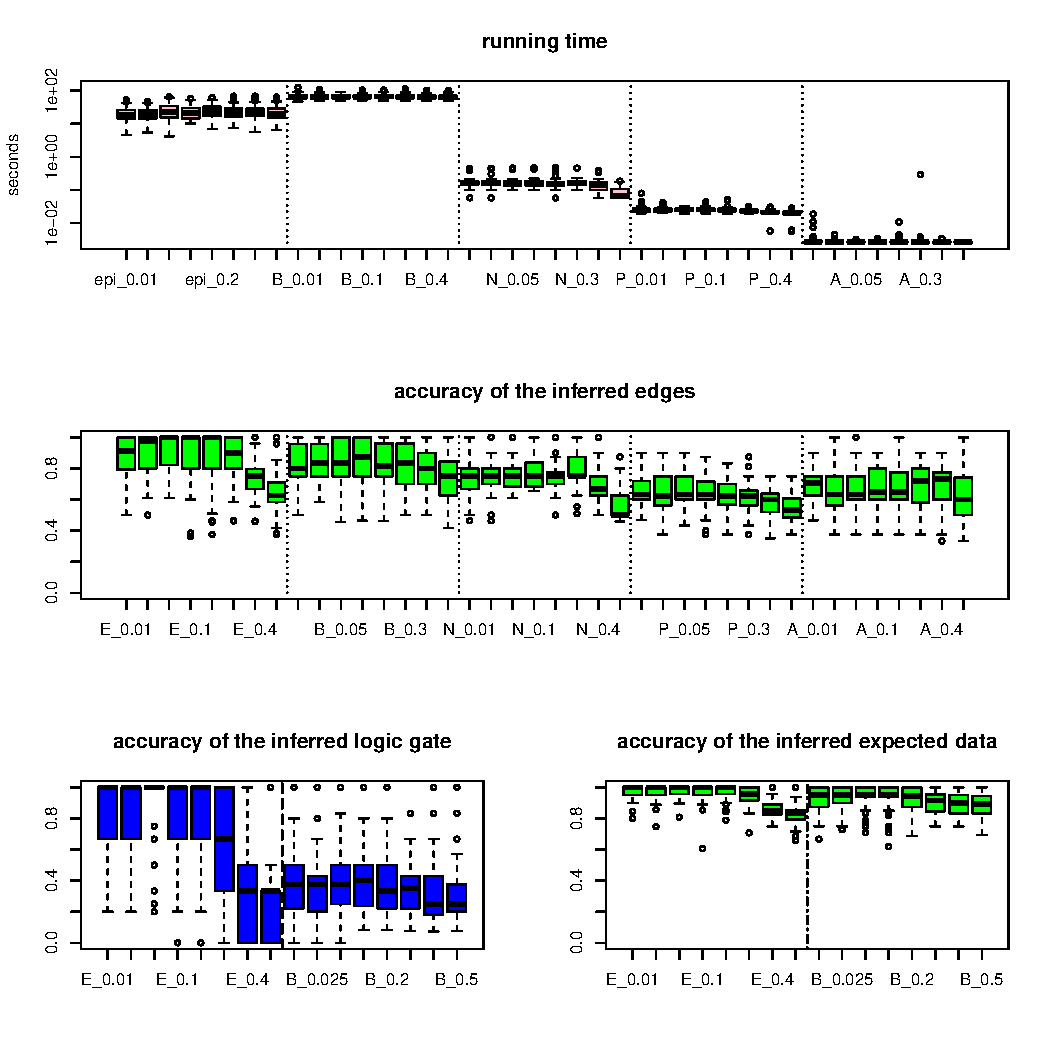
\includegraphics[width=\maxwidth]{figure/load_and_plot_simulation_results-1} 

}



\end{knitrout}

\section*{Yeast knockout screens}
In this section we analyse previously publish yeast knockout screens. The screens consist of gene expression data derived from double and single knockout mutants. We use epiNEM on each double mutant combined with each single mutant.

\subsection*{Wageningen et al., 2010} 

\begin{knitrout}
\definecolor{shadecolor}{rgb}{0.969, 0.969, 0.969}\color{fgcolor}\begin{kframe}
\begin{alltt}
\hlkwd{data}\hlstd{(wageningen)}

\hlstd{dataM} \hlkwb{<-} \hlstd{data[}\hlopt{-}\hlstd{(}\hlnum{1}\hlopt{:}\hlnum{2}\hlstd{), (}\hlnum{1}\hlopt{+}\hlstd{(}\hlnum{1}\hlopt{:}\hlstd{(}\hlnum{324}\hlopt{/}\hlnum{2}\hlstd{))}\hlopt{*}\hlnum{2}\hlstd{)]}

\hlstd{dataP} \hlkwb{<-} \hlstd{data[}\hlopt{-}\hlstd{(}\hlnum{1}\hlopt{:}\hlnum{2}\hlstd{), (}\hlnum{2}\hlopt{+}\hlstd{(}\hlnum{1}\hlopt{:}\hlstd{(}\hlnum{324}\hlopt{/}\hlnum{2}\hlstd{))}\hlopt{*}\hlnum{2}\hlstd{)]}

\hlstd{dataM} \hlkwb{<-} \hlstd{dataM[}\hlopt{-}\hlnum{1}\hlstd{, ]}

\hlstd{dataP} \hlkwb{<-} \hlstd{dataP[}\hlopt{-}\hlnum{1}\hlstd{, ]}

\hlstd{dataM} \hlkwb{<-} \hlkwd{apply}\hlstd{(dataM,} \hlkwd{c}\hlstd{(}\hlnum{1}\hlstd{,}\hlnum{2}\hlstd{), as.numeric)}

\hlstd{dataP} \hlkwb{<-} \hlkwd{apply}\hlstd{(dataP,} \hlkwd{c}\hlstd{(}\hlnum{1}\hlstd{,}\hlnum{2}\hlstd{), as.numeric)}

\hlstd{dataBin} \hlkwb{<-} \hlstd{dataM}

\hlstd{sig} \hlkwb{<-} \hlnum{0.05}

\hlstd{cutoff} \hlkwb{<-} \hlnum{0.7}

\hlstd{dataBin[}\hlkwd{which}\hlstd{(dataP} \hlopt{<} \hlstd{sig} \hlopt{&} \hlstd{dataP} \hlopt{>} \hlnum{0} \hlopt{&} \hlkwd{abs}\hlstd{(dataM)} \hlopt{>=} \hlstd{cutoff)]} \hlkwb{<-} \hlnum{1}

\hlstd{dataBin[}\hlkwd{which}\hlstd{(dataP} \hlopt{>=} \hlstd{sig} \hlopt{|} \hlstd{dataP} \hlopt{==} \hlnum{0} \hlopt{|} \hlkwd{abs}\hlstd{(dataM)} \hlopt{<} \hlstd{cutoff)]} \hlkwb{<-} \hlnum{0} \hlcom{# why do you throw away p-values with 0?}

\hlstd{dataBin} \hlkwb{<-} \hlstd{dataBin[}\hlopt{-}\hlkwd{which}\hlstd{(}\hlkwd{apply}\hlstd{(dataBin,} \hlnum{1}\hlstd{, max)} \hlopt{==} \hlnum{0}\hlstd{), ]}

\hlstd{genelist} \hlkwb{<-} \hlkwd{toupper}\hlstd{(}\hlkwd{c}\hlstd{(}\hlstr{'hsl1'}\hlstd{,} \hlstr{'cla4'}\hlstd{,} \hlstr{'gin4'}\hlstd{,} \hlstr{'swe1'}\hlstd{,} \hlstr{'hsl1.cla4'}\hlstd{))}

\hlstd{read_in_genes} \hlkwb{<-} \hlkwa{function}\hlstd{(}\hlkwc{genes}\hlstd{)\{}
    \hlkwd{return}\hlstd{(}\hlkwd{unlist}\hlstd{(}\hlkwd{lapply}\hlstd{(genes,} \hlkwa{function}\hlstd{(}\hlkwc{x}\hlstd{) \{}\hlkwd{paste}\hlstd{(x,} \hlstr{'.del.vs..wt.1'}\hlstd{,} \hlkwc{sep}\hlstd{=}\hlstr{''}\hlstd{)\})))}
\hlstd{\}}

\hlstd{single} \hlkwb{<-} \hlkwd{read_in_genes}\hlstd{(genelist)}

\hlkwd{colnames}\hlstd{(dataBin)} \hlkwb{<-} \hlkwd{gsub}\hlstd{(}\hlstr{".del.vs..wt"}\hlstd{,} \hlstr{""}\hlstd{,} \hlkwd{colnames}\hlstd{(dataBin))}

\hlkwd{colnames}\hlstd{(dataBin)} \hlkwb{<-} \hlkwd{gsub}\hlstd{(}\hlstr{".del"}\hlstd{,} \hlstr{""}\hlstd{,} \hlkwd{colnames}\hlstd{(dataBin))}

\hlstd{doubles} \hlkwb{<-} \hlkwd{colnames}\hlstd{(dataBin)[}\hlkwd{grep}\hlstd{(}\hlstr{"\textbackslash{}\textbackslash{}."}\hlstd{,} \hlkwd{colnames}\hlstd{(dataBin))]}

\hlstd{doubles} \hlkwb{<-} \hlkwd{sort}\hlstd{(doubles[}\hlopt{-}\hlkwd{grep}\hlstd{(}\hlstr{"vs"}\hlstd{, doubles)])}

\hlstd{doubles.genes} \hlkwb{<-} \hlkwd{unique}\hlstd{(}\hlkwd{unlist}\hlstd{(}\hlkwd{strsplit}\hlstd{(doubles,} \hlstr{"\textbackslash{}\textbackslash{}."}\hlstd{)))}

\hlstd{singles} \hlkwb{<-} \hlkwd{colnames}\hlstd{(dataBin)[}\hlopt{-}\hlkwd{grep}\hlstd{(}\hlstr{"\textbackslash{}\textbackslash{}."}\hlstd{,} \hlkwd{colnames}\hlstd{(dataBin))]}

\hlstd{singles} \hlkwb{<-} \hlkwd{unique}\hlstd{(}\hlkwd{sort}\hlstd{(singles))}

\hlstd{llmat} \hlkwb{<-} \hlstd{logicmat} \hlkwb{<-} \hlkwd{matrix}\hlstd{(}\hlnum{0}\hlstd{,} \hlkwd{length}\hlstd{(singles),} \hlkwd{length}\hlstd{(doubles))}

\hlkwd{rownames}\hlstd{(llmat)} \hlkwb{<-} \hlkwd{rownames}\hlstd{(logicmat)} \hlkwb{<-} \hlstd{singles}

\hlkwd{colnames}\hlstd{(llmat)} \hlkwb{<-} \hlkwd{colnames}\hlstd{(logicmat)} \hlkwb{<-} \hlstd{doubles}

\hlstd{globalgenes} \hlkwb{<-} \hlkwd{which}\hlstd{(}\hlkwd{apply}\hlstd{(dataBin,} \hlnum{1}\hlstd{, max)} \hlopt{==} \hlnum{1}\hlstd{)}

\hlcom{## for (i in doubles[set]) \{}
\hlcom{##     if (which(doubles %in% i) == 8) \{ next() \}}
\hlcom{##     print(i)}
\hlcom{##     doubles.singles <- unlist(strsplit(i, "\textbackslash{}\textbackslash{}."))}
\hlcom{##     egenes <- which(apply(dataBin[, which(colnames(dataBin) %in% c(i, doubles.singles))], 1, max) == 1)}
\hlcom{##     for (j in singles) \{}
\hlcom{##         print(j)}
\hlcom{##         if (j %in% doubles.singles) \{ next() \}}

\hlcom{##         dataTmp <- dataBin[, grep(paste(paste("^", c(i, j, doubles.singles), "$", sep = ""), collapse = "|"), colnames(dataBin))]}

\hlcom{##         if (path %in% "fixed_set") \{}
\hlcom{##             dataTmp <- dataTmp[egenes, ]}
\hlcom{##         \}}
\hlcom{##         if (path %in% "global") \{}
\hlcom{##             dataTmp <- dataTmp[globalgenes, ]}
\hlcom{##         \}}
\hlcom{##         if (path %in% "") \{}
\hlcom{##             dataTmp <- dataTmp[which(apply(dataTmp, 1, max) == 1), ]}
\hlcom{##         \}}

\hlcom{##         i1 <- which(singles %in% j)}
\hlcom{##         i2 <- which(doubles %in% i)}

\hlcom{##         if (!(is.null(dim(dataTmp)))) \{}

\hlcom{##             if (any(dataTmp[, j] != 0)) \{}

\hlcom{##                 epires <- epiNEM(dataTmp, method = "exhaustive")}

\hlcom{##                 tmp <- epires$logics}
\hlcom{##                 if ("OR" %in% tmp) \{}
\hlcom{##                     if (sum(epires$origModel[, j]) != 2) \{}
\hlcom{##                         tmp <- "NOEPI"}
\hlcom{##                     \} else \{}
\hlcom{##                         if (all(tmp %in% "OR")) \{}
\hlcom{##                             tmp <- "OR"}
\hlcom{##                         \} else \{}
\hlcom{##                             tmp <- tmp[which(!(tmp %in% "OR"))]}
\hlcom{##                         \}}
\hlcom{##                     \}}
\hlcom{##                 \}}

\hlcom{##                 logicmat[i1, i2] <- tmp}
\hlcom{##                 llmat[i1, i2] <- epires$score}

\hlcom{##             \} else \{}

\hlcom{##                 logicmat[i1, i2] <- "UNCON"}
\hlcom{##                 llmat[i1, i2] <- -Inf}

\hlcom{##             \}}

\hlcom{##         \} else \{}

\hlcom{##             logicmat[i1, i2] <- "UNCON"}
\hlcom{##             llmat[i1, i2] <- -Inf}

\hlcom{##         \}}

\hlcom{##     \}}

\hlcom{## \}}
\end{alltt}
\end{kframe}
\end{knitrout}

Plot results.









